% ----------------------------------------------------------
% Fundamentação Teórica
% ----------------------------------------------------------
\chapter{Fundamentação Teórica}\label{cap:fundamentacao-teorica}
% ----------------------------------------------------------

% ---
\section{Internet das Coisas}\label{sec:internet-das-coisas}
% ---

A área de IoT está em uma onda crescente, com um grande número de pessoas investindo nesse mercado, e um bom número de profissionais migrando para essa área. Há uma estimativa de que existem 19 milhões de profissionais trabalhando na indústria de desenvolvimento de software, e desses, 19\% trabalham em algum projeto relacionado a IoT. \cite{cw-iot}.

\begin{citacao}
''A próxima onda na era da computação será fora do domínio do ambiente de trabalho tradicional. No paradigma da IoT, muitos dos objetos que nos rodeiam estarão na rede de uma forma ou de outra. RFID (Radio Frequency Identification - Identificadores via Rádio Frequência) e as tecnologias de redes de sensores crescerão para enfrentar este novo desafio, em que os sistemas de informação e comunicação estão embutidos nos ambientes que nos rodeiam, de forma invisível.''. \cite{iot-article}. 
\end{citacao}

É notável o crescimento dessa área. Há uma expectativa de que, em 2020, o número de carros conectados a internet supere o número de carros não conectados, sendo esses carros possíveis de se comunicar com outros veículos e a infraestrutura das ruas, como os semáforos. \cite{goldmansachs-iot}. Segundo \citeonline{press-iot}, em 2014 a IoT substituiu a área da \textit{Big Data} como a tecnologia mais empolgante, ou seja, a tecnologia que mais pessoas iriam migrar e se interessar. 


% ---
\section{Raspberry Pi}\label{sec:raspberry-pi}
% ---

Quando se pesquisa algo sobre IoT é praticamente impossível não achar relação e links para \textit{Raspberry Pi}, Arduinos, e toda a área de \textit{DIY}. Atualmente existem três modelos, conforme a \autoref{table:comparativo-rpi} e \autoref{fig:todos-rpi}. 

\begin{figure}[htb]
	\caption{\label{fig:todos-rpi}\textit{RPi} A+ (esquerda), B+ (centro) e 2 Modelo B (direita).}
	\begin{center}
		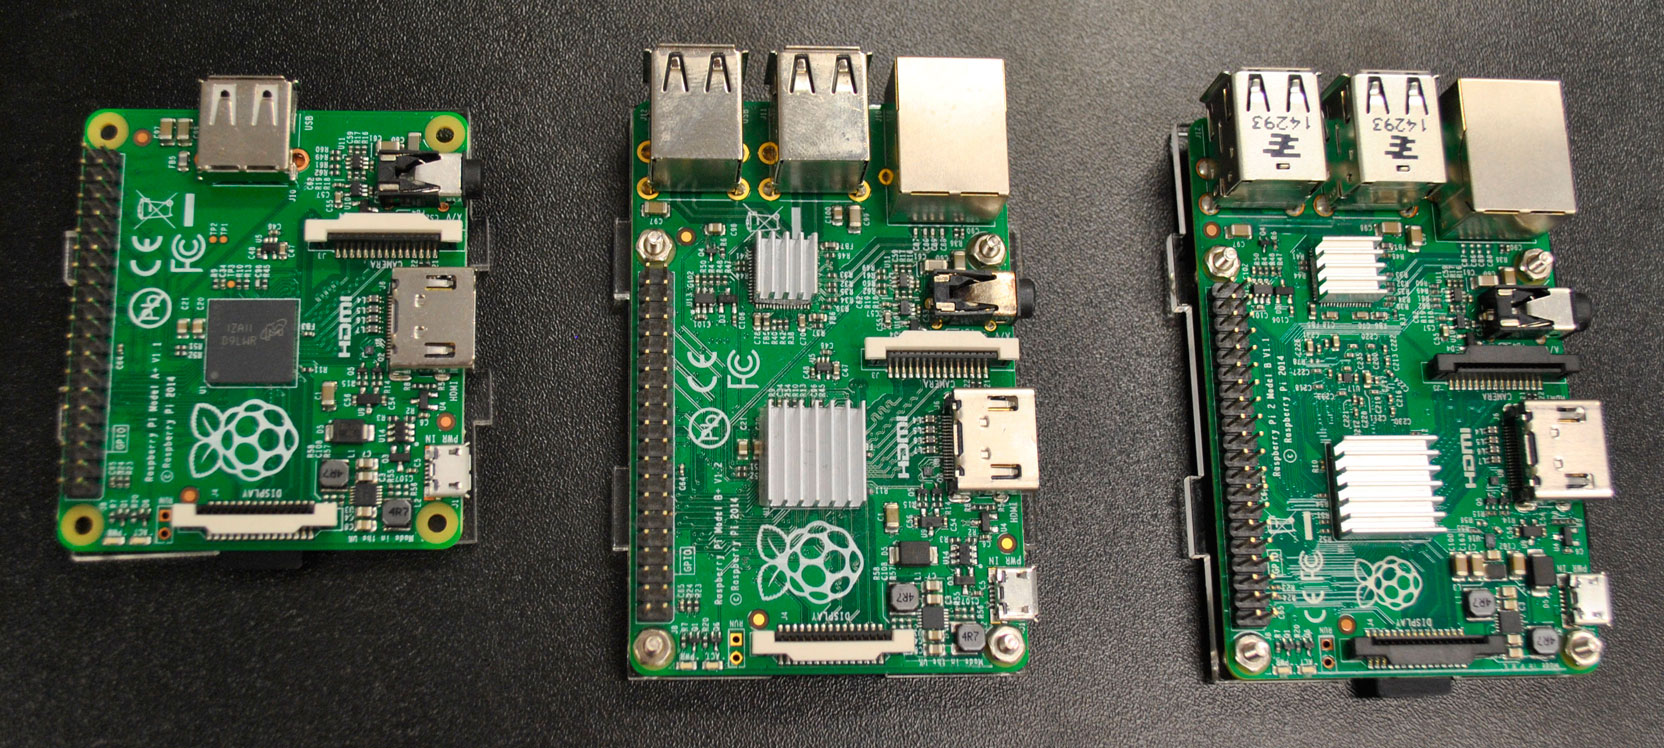
\includegraphics[width=0.8\textwidth]{img/rpi-modelos.jpg}
	\end{center}
	\legend{Fonte: elaborado pelo autor}
\end{figure}

\begin{table}[htb]
	\IBGEtab{%
  		\caption{Comparativo entre os modelos de \textit{Raspberry Pi}}%
  		\label{table:comparativo-rpi}
	}{%
  		\begin{tabular}{cccc}
	  		\toprule
	 			Versão & A+ & B+ & 2 Modelo B \\
  			\midrule \midrule
				Processador & ARMv6 single core & ARMv6 single core & ARMv7 quad core \\
			\midrule
				Velocidade CPU & 700 MHz single-core & 700 MHz single-core & 900 MHz quad-core \\
			\midrule 
				Memória RAM & 256 MB & 512 MB & 1 GB \\
  			\midrule 
				Portas USB & 1  & 4  & 4 \\
			\midrule 
				\textit{Ethernet} & Não & Sim  & Sim \\
  			\bottomrule
		\end{tabular}%
	}{%
  		\fonte{\cite{rpiversion-table}}%
  	}
\end{table}

Segundo \citeonline{raspberrypi-rpi}, esse pequeno dispositivo foi criado com intuito de ser utilizado por crianças e pessoas carentes do mundo todo para aprender programação e computação. É facilmente configurável, utilizando um cartão de memória como HD para o sistema operacional e dados.

Por meio de suas portas de entrada e saída digitais é possível conectar uma gama ampla de sensores, atuadores, componentes eletrônicos, ficando a cargo do programador e criador do projeto escolher como esses pinos serão conectados e aproveitados. Atualmente existem diversos módulos para expandir os meios de comunicação entre diferentes \textit{devices}, e um deles é via \textit{bluetooth}.

Atualmente existem diferentes sistemas operacionais portados para o \textit{RPi}.

\begin{alineas}
	\item \textbf{Raspbian}: baseado na distribuição \textit{Linux} chamada \textit{Debian}. Atualmente é a suportada oficialmente pela \textit{RPi Foundation}. \cite{rpi-download};
	\item \textbf{Ubuntu Mate}: baseado na distribuição \textit{Linux} chamada \textit{Ubuntu}, juntamente com o software \textit{MATE Desktop} para gerenciamento de janelas. \cite{ubuntu-mate};
	\item \textbf{Snappy Ubuntu Core}: distribuição \textit{Linux} voltada a \textit{cloud} e dispositivos. \cite{snappy-ubuntu};
	\item \textbf{Windows 10 for IOT Core}: versão do \textit{Windows} 10 da \textit{Microsoft} para dispositivos voltados a internet das coisas. \cite{windows10-iot}.
\end{alineas}

% ---
\section{Bluetooth Low Energy}\label{sec:ble}
% ---

A tecnologia do \textit{bluetooth} vem sendo amplamente utilizada, principalmente após a criação da versão 4.0, ou \textit{BLE} (\textit{Bluetooth Low Energy} - Bluetooth de Baixa Energia), por conta de ter um baixíssimo gasto energético, podendo preservar a bateria do dispositivo que a utiliza. O \textit{BLE} faz parte da tecnologia nomeada \textit{Bluetooth Smart} inteligente e eficiente energeticamente, voltada para \textit{devices} que usam pequenas fontes de energia. \cite{bluetooth-smart}.

O \textit{BLE} possui similaridades com a versão clássica do \textit{bluetooth}. Ambos utilizam o espectro de frequências de 2.4 GHz (mesmo utilizado pelas redes \textit{WiFi}), mesma modulação GFSK e velocidade de 1 Mbps, porém a indexação de ambos é diferente. A versão clássica possui 79 canais, e a \textit{BLE} possui 40 canais. Além disso, os canais são espaçados de forma diferente, conforme \autoref{table:ble-physical}. \cite{ble-packets}.

\begin{table}[htb]
	\IBGEtab{%
  		\caption{\textit{BLE Physical Layer}}%
  		\label{table:ble-physical}
	}{%
  		\begin{tabular}{ccc}
	  		\toprule
	 			  & BLE & Classic \\
  			\midrule \midrule
				Modulação & GFSK 0.45 a 0.55 & GFSK 0.28 a 0.35 \\
			\midrule
				Velocidade de Transferência & 1 Mbit/s & 1 Mbit/s \\
			\midrule 
				Canais & 40 & 79 \\
  			\midrule 
				Espaçamento & 2 MHz & 1 MHz \\
  			\bottomrule
		\end{tabular}%
	}{%
  		\fonte{\cite{ble-packets}}%
  	}
\end{table}

O espectro de 2.4 GHz para \textit{bluetooth} se extende de 2402 MHz a 2480 MHz, e os canais 37, 38 e 39 (últimos três) são específicos para anúncio (\textit{advertisement}), conforme \autoref{fig:banda-channels}.  \cite{ble-packets}. 

\begin{figure}[htb]
	\caption{\label{fig:banda-channels}Separação da banda 2.4 GHz para bluetooth e WiFi.}
	\begin{center}
		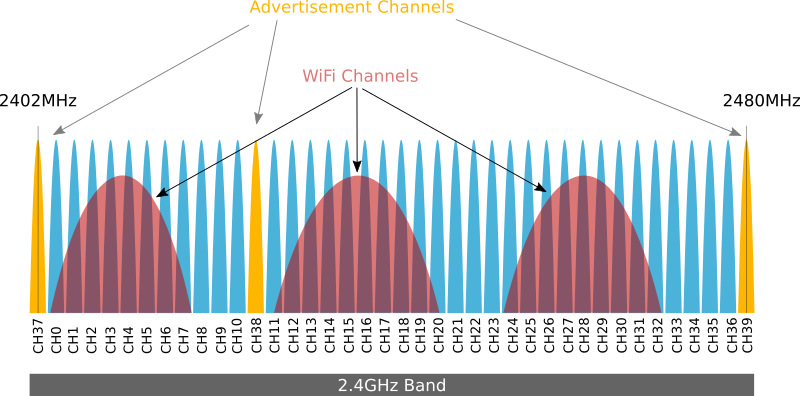
\includegraphics[width=0.7\textwidth]{img/banda-2-4.png}
	\end{center}
	\legend{Fonte: \cite{ble-packets}}
\end{figure}

Interessante notar que esses canais estão posicionados em forma bastante estratégica, no começo, final e meio da banda de 2.4 GHz, com a finalidade de aumentar a eficácia, evitando todos os canais ficarem lotados ou com muita interferência. \cite{ble-packets}. 

Os \textit{BLE Advertisement Packets}, ou pacotes de anúncio \textit{BLE} é uma das formas de conexão do \textit{Bluetooth Smart}. Por meio dos anúncios, um \textit{device} transmite pacotes para todos que estão a sua volta, sem necessariamente necessitar de uma conexão direta entre somente outro dispositivo.

Um \textit{BLE Advertisement Packet} é formado conforme \autoref{fig:ble-adv-packet}. O preâmbulo, \textit{access address} e CRC são informações para formação do pacote. Os dados estão de fato dentro do PDU (\textit{Packet Data Unit}). O cabeçalho de 2 bytes informa o tamanho do \textit{payload} (carga de dados), além de informações relevantes como tipo do pacote, tipo de mensagem enviada, entre outros. \cite{ble-packets}.

\begin{figure}[htb]
	\caption{\label{fig:ble-adv-packet}Modelo de \textit{BLE Advertising Packet}.}
	\begin{center}
		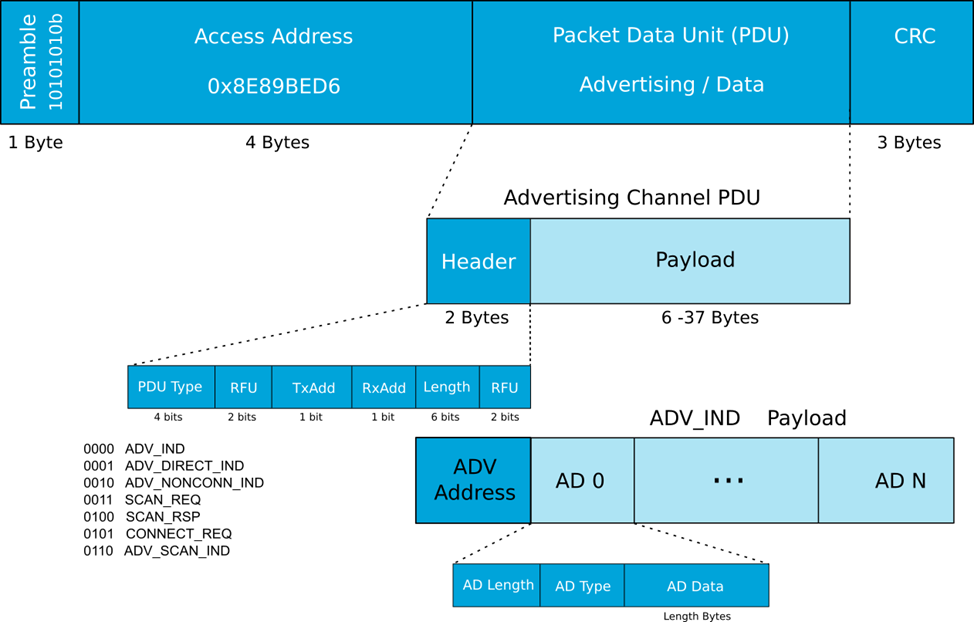
\includegraphics[width=0.8\textwidth]{img/ble-adv-packet.png}
	\end{center}
	\legend{Fonte: \cite{ble-packets}}
\end{figure}

O importante do \textit{BLE Advertising Packet} é o tipo de anúncio feito, ou quais são as informações do pacote. \citeonline{gap-ble} apresenta uma tabela com os possíveis valores e também o significado de cada uma. Por exemplo, o valor 0xFF significa que o pacote contém dados específicos do fabricante, ou seja, existe a flexibilidade de manipular o pacote da forma que for precisa, contanto que mantenha a estrutura original de 6 a 37 bytes de \textit{payload}, conforme \autoref{fig:ble-adv-packet}. \cite{ble-packets}.

% ---
\section{Beacon}\label{sec:beacon}
% ---

Os \textit{beacons} são pequenos sensores que são capazes de identificar objetos com precisão dentro de ambientes fechados. \cite{teixeira-beacon}.

\begin{citacao}
Como muitos espaços fechados (restaurantes, museus, shopping centers, casas de show) possuem estrutura metálica ou utilizam algum tipo de metal em sua construção, é comum que o sinal de GPS fique enfraquecido quando os usuários estão dentro daquele local. Nesse caso, os \textit{Beacons} são uma ótima solução: um hardware relativamente barato, e pequeno o suficiente para ser plugado na parede ou instalado sobre um balcão. \cite{teixeira-beacon}.
\end{citacao}

\begin{figure}[htb]
	\caption{\label{fig:beacon-mpact}Modelo de \textit{beacon} proprietário: MPact, da Zebra Technologies Corporation.}
	\begin{center}
		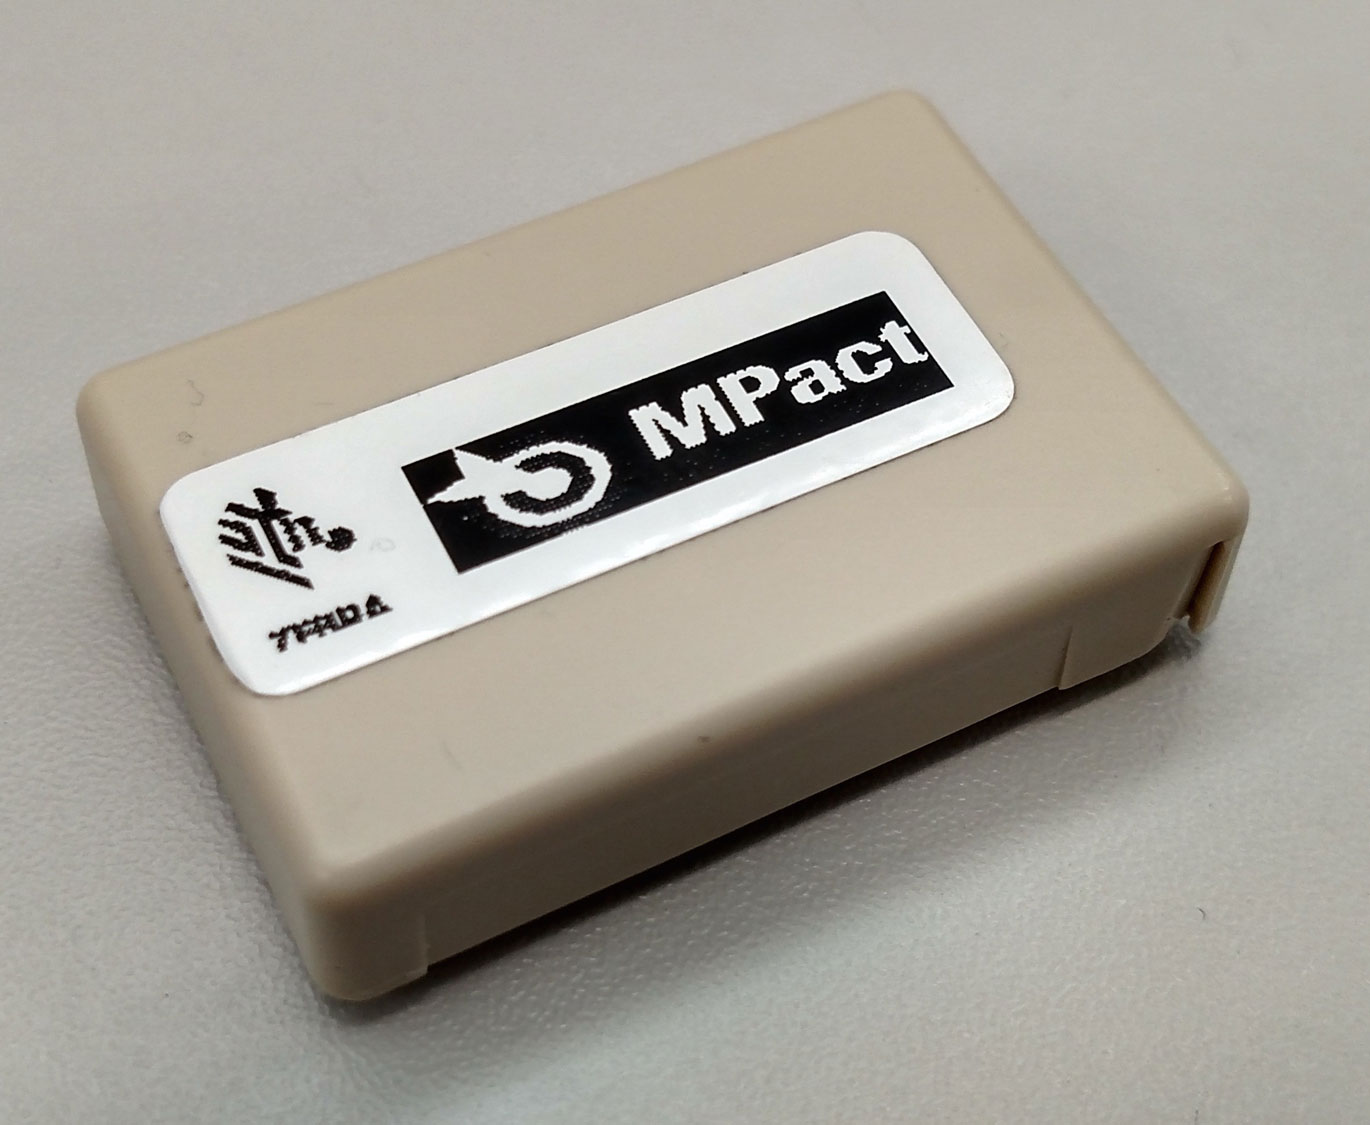
\includegraphics[width=0.6\textwidth]{img/beacon-mpact.jpg}
	\end{center}
	\legend{Fonte: elaborado pelo autor}
\end{figure}

Segundo \citeonline{teixeira-beacon}, os \textit{beacons} utilizam o \textit{BLE} para detectar um dispositivo próximo e transmitir seu identificador único e avisar que está ali presente. \citeonline{teixeira-beacon} também diz que os \textit{beacons} não são inteligentes, toda a interação deve depender do dispositivo que recebe a informação do identificador único.

Atualmente os usos de \textit{beacons} estão restritos a aplicativos em smartphones realizando a leitura e interagindo com o usuário, porém existem ainda diversas áreas a serem exploradas, e um bom exemplo são as casas inteligentes. Segundo \citeonline{grothaus-smarthomes}, a \textit{Apple} está apostando em um kit de desenvolvimento (\textit{HomeKit}) que permita aos desenvolvedores interagirem com \textit{smart devices} presentes no ambiente.

% ---
\subsection{\textit{iBeacon}}\label{sec:ibeacon}
% ---

O protocolo \textit{iBeacon} foi apresentado pela Apple juntamente com o iOS 7, versão de seu sistema operacional para dispositivos móveis. É uma tecnologia baseada nos \textit{beacons}, porém adaptada para as necessidades e aplicações de seu sistema móvel.

A Apple adaptou o pacote genérico de \textit{beacon} para transmitir três dados:

\begin{alineas}
	\item \textbf{UUID}: Identificador único formado de 16 bytes (128 bits). Focado em ser único para cada aplicação. Cada aplicação deve ter um único UUID;
	\item \textbf{\textit{Major}}: Identificador de 2 bytes que identifica uma sub-região grande. Usado, por exemplo, para dividir as lojas de um grande varejista;
	\item \textbf{\textit{Minor}}: Identificador de 2 bytes que identifica uma sub-divisão de região, ou seja, uma região menor que o Major.
\end{alineas}

Um exemplo de aplicação é citado na \autoref{table:stores-apple}. Utiliza-se um único UUID para todas as lojas, um número \textit{Major} por loja e um \textit{Minor} por departamento, podendo este último ser repetido entre as lojas.

\begin{table}[htb]
	\IBGEtab{%
  		\caption{Exemplo de aplicação}%
  		\label{table:stores-apple}
	}{%
  		\begin{tabular}{cccc}
	  		\toprule
	 			Localização da Loja & São Francisco & Paris & Londres \\
  			\midrule
				UUID & \multicolumn{3}{c}{D9B9EC1F-3925-43D0-80A9-1E39D4CEA95C} \\
			\midrule
				\textit{Major} & 1 & 2 & 3 \\
			\midrule 
				\textit{Minor} (Roupas) & 10 & 10 & 10 \\
  			\midrule 
				\textit{Minor} (Utilidades Domésticas) & 20 & 20 & 20 \\
			\midrule 
				\textit{Minor} (Automotivo) & 30 & 30 & 30 \\
  			\bottomrule
		\end{tabular}%
	}{%
  		\fonte{\cite{ibeacon-apple}}%
  	}
\end{table}

O pacote \textit{BLE} utilizado pela tecnologia iBeacon pode ser visto na \autoref{fig:ibeacon-packet}. Segundo \citeonline{arm-beacons}, o prefixo determinado para o protocolo \textit{iBeacon} é:

\begin{alineas}
	\item \textit{\textbf{Adv Flags}}: determinam que é um pacote \textit{BLE} de descobrimento geral, e que somente transmite e não permite conexões;
	\item \textit{\textbf{Adv Header}}: determinam que os próximos 26 bytes serão a carga de dados (\textit{payload} de fato). Sempre será 0x1AFF;
	\item \textit{\textbf{Company ID}}: indica que é o ID da Apple junto com a Bluetooth SIG. Essa informação que faz ser dependente da Apple. Sempre será 0x004C;
	\item\textit{\textbf{iBeacon Type}}: ID secundário utilizado por todos iBeacons que identificam ser um \textit{beacon} de proximidade. Sempre será 0x02;
	\item\textit{\textbf{iBeacon Length}}: identifica quantos bytes terão em seguida. Sempre será 0x15, ou 21 bytes.
\end{alineas}

\begin{figure}[htb]
	\caption{\label{fig:ibeacon-packet}\textit{Payload} do pacote iBeacon.}
	\begin{center}
		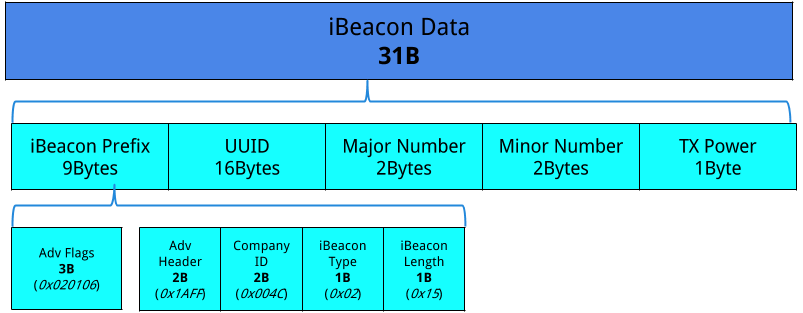
\includegraphics[width=1\textwidth]{img/ibeacon-packet.png}
	\end{center}
	\legend{Fonte: \cite{arm-beacons}}
\end{figure}

Os \textit{iBeacons} foram criados com intuito de serem descobertos por smartphones. Um exemplo de aplicação é uma cafeteria com um \textit{iBeacon} no balcão próximo ao caixa. Quando um consumidor entra na loja e chega próximo ao caixa, um aplicativo em seu celular identifica o \textit{iBeacon} pela sua UUID, identifica pelo \textit{Major} que se trata da cafeteria número 12 e encontra uma promoção com o \textit{Minor} de número 26. Em seguida, apresenta uma notificação ao usuário uma promoção e também um cupom válido de desconto para usar no caixa. \cite{arm-beacons}.

Uma outra aplicação interessante citada por \citeonline{arm-beacons} é a possibilidade do smartphone transmitir pacotes \textit{iBeacon}, sem necessidade de um hardware externo. Dessa forma, pode-se por exemplo automatizar o check-in em um evento e rastrear o movimento dos usuários entre os estabelecimentos.

% ---
\subsection{Outros Protocolos}\label{sec:outros-protocolos}
% ---

Existem mais protocolos baseados na tecnologia \textit{beacon}. Dois se destacam por ser abertos e passíveis de alterações: \textit{AltBeacon} e \textit{Eddystone}, este último criado pela Google. O \textit{AltBeacon} possui um modelo bastante parecido com o \textit{iBeacon}, porém com possibilidade de alterar o número do fabricante, ter possibilidade de código de \textit{beacons} diferentes, e também a possibilidade do fabricante colocar sua informação ao final do pacote, conforme \autoref{fig:altbeacon-packet} \cite{arm-beacons}.

Segundo \citeonline{eddystone-google}, o protocolo \textit{Eddystone} possui três modos de funcionamento:
\begin{alineas}
	\item \textit{Eddystone}-UID: transmite um \textit{beacon} ID, composto de 10 bytes identificando um grupo de \textit{beacons} e  6 bytes identificando um único \textit{beacon};
	\item \textit{Eddystone}-URL: transmite um link comprimido, para que o cliente possa acessar um site na internet;
	\item \textit{Eddystone}-TLM: transmite informações de telemetria sobre o \textit{beacon}, como por exemplo voltagem da bateria, temperatura e quantos pacotes foram enviados.
\end{alineas}

\begin{figure}[htb]
	\caption{\label{fig:altbeacon-packet}Pacote do \textit{AltBeacon}.}
	\begin{center}
		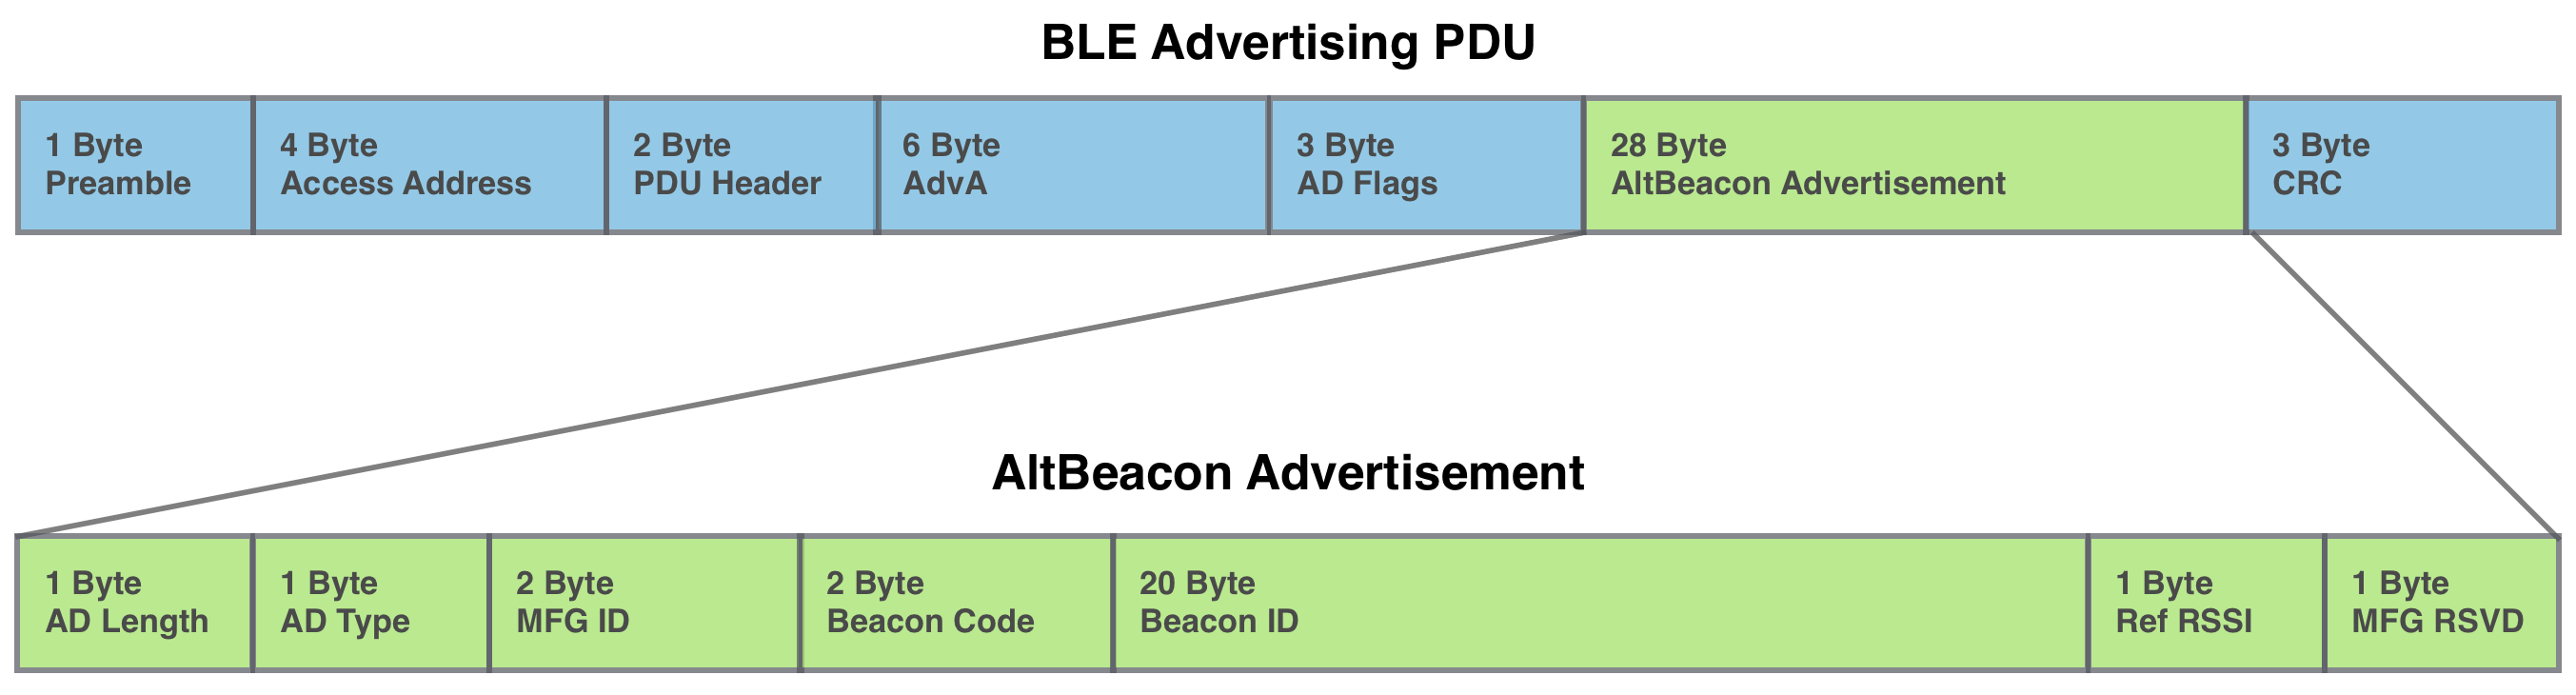
\includegraphics[width=1\textwidth]{img/altbeacon-packet.png}
	\end{center}
	\legend{Fonte: \cite{arm-beacons}}
\end{figure}

% ----------------------------------------------------------